\chapter{Cahier des charges}

\section{Introduction}

La plupart des langages de programmation offrent des capacités similaires pour stocker des nombres et effectuer des calculs. Ces langages permettent, entre autres, d'utiliser  des nombres réels.

Ces nombres réels ont tout de même des limitations. Ils sont limités au domaine du réel. De plus, les nombres à virgule flottante sont souvent inexacts. Par conséquent, lorsque les erreurs s'accumulent, le résultat d'un calcul peut être très éloigné de la réponse exacte.

Pourtant, d'autres alternatives existent. Les nombres complexes sont couramment utilisés en mathématique et en physique. Ils peuvent être utilisés pour simplifier des réponses utilisant des racines de nombres négatifs ou pour combiner deux quantités réelles telles que la tension et l'intensité en électricité. Quant à eux, les nombres réels peuvent aussi être représentés différemment. Les \textbf{universal numbers} (\textbf{unums}) sont une représentation alternative possible dont la dernière version est expliquée dans l'article \textit{Beating Floating Point at its Own Game: Posit Arithmetic} \cite{posit}.


\section{Contexte}

En Java, aucun type ni aucune classe dans le JDK permet de gérer des nombres complexes ou des unum, mais il est possible de l'implémenter soi-même. Des librairies pouvant gérer ces éléments peuvent déjà exister.

La première solution pour ajouter ces fonctionnalités et de créer de nouvelles classes: une classe pour les nombres complexes et une classe pour les unums. Ensuite, il faut écrire le code en utilisant directement ces classes. Pour changer le type de calculs effectué (ex: nombre complexe $\rightarrow$ nombre réel), il faut changer le code source de l'application.

COJAC \cite{COJAC} est une librairie Java permettant de modifier les capacités arithmétiques d'un programme Java sans en modifier le code. Elle utilise l'API d'instrumentation et peut transformer les classes et méthodes au runtime pour changer le type de calcul effectué. Ainsi, pour changer le type de calculs effectué (ex: nombre réel $\rightarrow$ nombre complexe), il faut seulement changer l'argument donné à COJAC \cite{COJAC} lors du démarrage de l'application. Ceci ne demande aucune modification dans l'application de l'utilisateur.

\section{Objectifs}

Le but de ce projet est d'ajouter deux nouvelles fonctionnalités à COJAC \cite{COJAC}. COJAC devra permettre de remplacer automatiquement les nombres à virgules flottantes par deux nouveaux types numériques.

\subsection{Intégration des nombres complexes}

Une option de COJAC permettra de changer le comportement des calculs dans l'application de l'utilisateur. Les nombres à virgules flottantes (\textit{float} et \textit{double}) seront remplacés, au runtime, par des nombres complexes. Les opérations arithmétiques telles que l'addition, la soustration, etc. devront être adaptées. De plus, les méthodes souvent utilisées de la librairie standard devront également pouvoir fonctionner. Par exemple, la méthode \textit{Math.sqrt} devra permettre de retourner la racine carrée d'un nombre négatif.

Voici un exemple sans les nombres complexes:
\begin{minted}{Java}
double val = Math.sqrt(-1); // = NaN
val = val * val; // = NaN;
\end{minted}

Avec les nombres complexes, on obtient le résultat suivant:
\begin{minted}{Java}
double val = Math.sqrt(-1); // = i
val = val * val; // = -1;
\end{minted}

\subsection{Intégration des unums}

Une option de COJAC permettra de changer le format de stockage et de calculs des nombres réels. Les unums seront utilisés à la place de la virgule flottante. Par conséquent, les opérations arithmétiques devront être redéfinies pour fonctionner avec ce nouveau format de stockage. Il faudra probablement utiliser JNI pour accéder à une librairie C/C++ permettant d'utiliser les unums, mais d'autres approches restent possibles.

\subsection{Démonstration des deux fonctionnalités}

Des programmes de démonstrations seront réalisés pour montrer ces deux fonctionnalités. Ces démonstrations doivent montrer l'utilité et les avantages de cette approche.

\begin{minipage2}
\section{Objectifs secondaires}

D'autres ajouts de fonctionnalités ou modifications permettraient d'améliorer ce projet.

\subsection{Mise à jour des librairies}

COJAC \cite{COJAC} utilise plusieurs librairies dont les versions sont désormais obsolètes. Il vaut mieux mettre à jour les versions avant de rencontrer des problèmes à cause de versions trop anciennes. Cependant, COJAC \cite{COJAC} devra garantir une compatibilité pour Java 8+.
\end{minipage2}

\subsection{Tests de performance}

Lorsque les fonctionnalités de remplacement des nombres à virgule flottante par des nombres complexes et des unums, il restera encore un aspect inconnu qui est pourtant important pour décider de l'utilité de cette fonctionnalité: les performances. Pour cette raison, des tests de performance peuvent aussi être ajoutés pour tester l'efficacité de l'implémentation.

\subsection{Documentation et promotion}

COJAC possède une documentation pour l'utiliser et des vidéos pour expliquer l'utilité de certaines fonctionnalités. Il serait possible de documenter les nouvelles fonctionnalités ajoutées, de réaliser une vidéo pour montrer l'utilité de ces vidéos ou encore de compléter la documentation actuelle.

\subsection{Comparaison des approches wrappers et behaviours}

Deux approches sont possibles pour implémenter de nouvelles fonctionnalités dans COJAC:
\begin{itemize}
    \item Behaviour: les opérations sur les floats et les doubles sont simplement remplacées par un appel de méthode. Ainsi, il est possible de changer le comportement de ceux-ci. Dans ce projet, il serait possible de mettre la partie réelle et la partie imaginaire dans un double et de modifier les opérations qui les utilisent.
    \item Wrapper: les floats et les doubles peuvent être remplacés par un objet (wrapper). Ce qui permet d'ajouter plus d'éléments dans le wrapper.
\end{itemize}

\subsection{Améliorations diverses}

Toute autre amélioration à la base de code existante est aussi le bienvenu. Voici quelques exemples d'améliorations qui pourraient être effectuées:
\begin{itemize}
    \item Ajout d'un CI sur GitLab pour vérifier les tests et compiler le JAR.
    \item Ajout d'un logger pour améliorer la gestion des logs.
    \item Améliorer l'architecture du projet.
    \item Améliorer la documentation du code.
    \item Faire les TODO présents dans le code.
\end{itemize}

\section{Tâches}

Cette section détaille les tâches qui devront être effectuées pour réaliser chacun des objectifs définis précédemment.

\subsection{Intégration des nombres complexes}

Les tâches suivantes seront effectuées pour réaliser cet objectif:
\begin{itemize}
    \item Analyse des implémentations existantes.
    \item Analyse de COJAC et de comment intégrer un nouveau type.
    \item Analyse des nombres complexes.
    \item Concevoir l'intégration des nombres complexes.
    \item Intégrer des nombres complexes.
    \item Tester l'intégration des nombres complexes.
\end{itemize}

\subsection{Intégration des unums}

Les tâches suivantes seront effectuées pour réaliser cet objectif:
\begin{itemize}
    \item Analyse des implémentations existantes.
    \item Analyse de COJAC et de comment intégrer un nouveau type.
    \item Analyse des unums.
    \item Choix d'une variante d'unum à implémenter.
    \item Concevoir l'intégration des unums.
    \item Intégrer des unums.
    \item Tester l'intégration des unums.
\end{itemize}

\subsection{Démonstration}

Les tâches suivantes seront effectuées pour réaliser cet objectif:
\begin{itemize}
    \item Concevoir les démonstrations.
    \item Réaliser les démonstrations.
\end{itemize}

\subsection{Mise à jour des librairies}

Les tâches suivantes seront effectuées pour réaliser cet objectif:
\begin{itemize}
    \item Chercher les mises à jour de chaque librairie.
    \item Regarder les changements avec la nouvelle version.
    \item Modifier la version et adapter le code.
    \item Tester les modifications.
\end{itemize}

\subsection{Tests de performance}

Les tâches suivantes seront effectuées pour réaliser cet objectif:
\begin{itemize}
    \item Analyser les tests de performance actuels.
    \item Réaliser les tests de performance.
    \item Synthétiser les tests de performance.
\end{itemize}

\begin{landscape}
\section{Planification}
La figure \ref{fig:gantt} montre le diagramme de Gantt avec la liste des jalons et des tâches durant le projet. Ce travail dure du 31 mai au 16 juillet 2021.
\begin{figure}[h!]
   \centering
    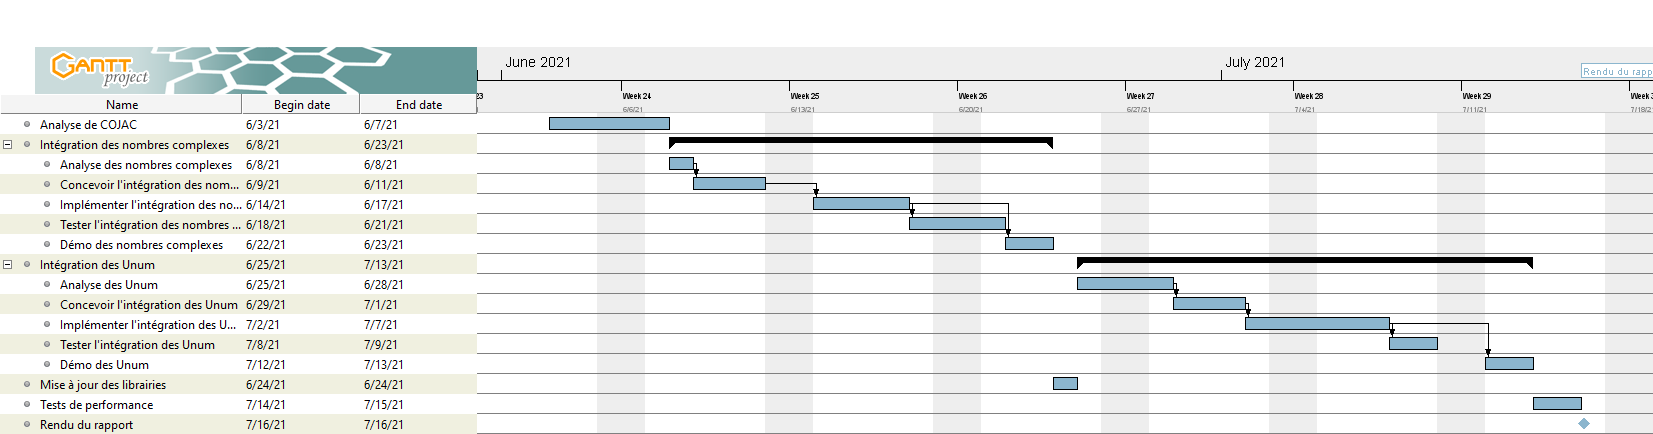
\includegraphics[width=0.84\linewidth]{specifications/planning.png}
    \caption{Diagramme de Gantt}
    \label{fig:gantt}
\end{figure}

D'autres dates importantes sont également prévues plus tard dans l'année pour présenter ce projet.

\begin{table}[ht]
    \begin{tabularx}{\columnwidth}{ | X | p{8em} |}
        \hline
        \textbf{Activité} & \textbf{Date limite} \\
        \hline
        Rendu du poster & 27.08.2021 \\
        Exposition du travail de bachelor & 03.09.2021 \\
        Défense orale & 06-08.09.2021 \\
        \hline
    \end{tabularx}
\end{table}

\end{landscape} 